\documentclass[12pt]{article}
\usepackage{mathptmx}
%\usepackage{kantlipsum}
\usepackage[margin=1in]{geometry}
\usepackage{setspace}
\usepackage{graphicx}
\usepackage{etoolbox}
\AtBeginEnvironment{quote}{\singlespacing\small}

\usepackage[style=apa, 
            language=american, 
            backend=biber, 
            natbib=true, 
            hyperref=true, 
            uniquelist=true]{biblatex}

\DeclareLanguageMapping{american}{american-apa}
\addbibresource{proposal_bibliography.bib}

\title{Detecting ``Fake News" on Facebook}
\author{Hannah Eyre \and Zane Zakraisek}
\begin{document}
\maketitle
\setstretch{1.2}

The term ``Fake News" gained popularity during the United States' 2016 Presidential Election to describe a rapidly spreading phenomena of news articles deliberately spreading false information and hoaxes, often through attention grabbing headlines or headlines that resemble legitimate sources \citep{guardian}. It became particularly notorious on social media sites and Facebook in particular. Here, the top 20 articles from fake news sites and hyperpartisan blogs garnered more user interaction between August 1st and election day on November 8th than the top 20 articles from a variety of established news sources. These included {\it The New York Times}, {\it Washington Post}, {\it Business Insider}, and Fox News \citep{buzzfeed}.

\textit{FactCheck.org}, part of the Annberg Public Policy Center at the University of Pennsylvania, breaks down how an individual can identify fake news into eight parts \citep{factcheck}:
\begin{quote}
\begin{enumerate}
\item Consider whether the source is credible.
\item Read beyond the headline.
\item Check whether the author is credible or real.
\item Check whether the article is recent.
\item Check whether the article is a joke or satire.
\item Consider your own biases and how they affect your judgment.
\item Check supporting sources (if any) and make sure they abide by the same rules.
\item Ask experts or fact-checking sites.
\end{enumerate}
\end{quote}

Rapidly spreading fake news articles have a range of consequences, one instance culminating in a gunman attacking a Washington, DC pizza parlor over allegations of a satanic child sex abuse ring centered around John Podesta, Hillary Clinton's 2016 campaign manager, in a conspiracy called ``Pizzagate" \citep{pizzagate}. Various politicians and government agencies in the United States and internationally have voiced opinions on what qualifies as fake news, and more importantly, what to do about it. However, up to this point, no consensus has been reached. Facebook was initially reluctant to admit there was any problem with fake news on their website, however, Facebook's CEO Mark Zuckerberg has since released a statement describing how they plan to deal with fake news in the future, including renaming the phenomenon ``false news" \citep{zuckerberg}.

As an increasingly global and hotly contested issue, we would like to to explore what responsibility Facebook has in regards to these eight points. We will discuss whether they have a responsibility to develop tools to detect fake news based off these guidelines and, if these tools exist, whether they should be used to remove content from the site. We will be using two particular examples, Pizzagate as mentioned above and conspiracies spread in the hours and days following the Las Vegas shooting. We feel that Pizzagate is a primary example of what happens when fake news reaches a critical mass of interest online, having large followings on Reddit, 4chan, Breitbart and Infowars that actively encouraged ``citizen investigation". Additionally, the Las Vegas shooting conspiracies are a group of examples of the rapid spreading of fake news, particularly when real information is unavailable or unclear. In the early morning hours following the October 1, 2017 shooting, the website 4chan organized a successful effort to manipulate trending topics across the web and spread misinformation before real information was distributed.

The other primary focus of our analyzation comes from a utilitarian perpective. When analyzing any issue, it's important to define what framework you're working in, along with what premises your arguments are based on. During our analysis of the Facebook's role in moderating fake news, we'll be working under a utilitarian framework. In particular, our primary goal is reducing the negative utility fake news brings about. As we examine role that fake news has played in the events mentioned, it is evident that fake news results in a negative utility for Facebook's users. News on Facebook has the potential to result in positive utility, and like fake news, it is due to the rapid spread and wide range of people reached. We believe access to a variety of news sources is an important part of interacting with social media and results in a greater positive utility than fake news causes negative. Because of this, we believe removing news in general from Facebook would increase negative utility overall. As a result, we find that it is far more important to try to minimize the corresponding negative utility caused by fake news.

As we address each of these eight points mentioned above, the format shall be as follows. We'll first examine the status quo where Facebook has not publicly addressed efforts made to combat fake news and how that is affecting users. Next, we'll examine the outcome if Facebook chose to implement a fake news monitoring system using this technique. Lastly, we'll weigh the different utilities and select the one that we feel minimizes the negative utility. In addition to this, we'll also be examining whether or not the method is technically feasible to implement with current technology.

\section{Credible sources: Sites and Authors}
The first method in combating the spreading of fake news is to check whether or not the article in question comes from a credible source. This involves not just the author, but the site as well. To start off, we'll examine the utility if Facebook chose \textit{not to} implement this source credibility check. Although Facebook implements a very light form of censorship (citep), the scenario would be quite similar to how Facebook currently monitors articles, which is very little. While most articles that Facebook news feeds show users are based off topics that they've shown interest in, nearly every Facebook user has probably been shown an article from an underground website that someone on their friends list has liked or shared. If Facebook didn't implement source credibility prioritization, then the effect of one person sharing an article like this could have quite a negative outcome. The article in question can easily make its way to hundreds of people. In most cases, this has the effect of increasing the amount of negative utility, as most fake news articles are spread with negative motivations in mind.

Now assume Facebook was to implement source credibility prioritization. In this same scenario, if someone was to like or share an article, Facebook could first check its feedback for that particular site and/or author. If there is enough feedback, and the score is negative, Facebook could deprioritize the article on other people's news feeds by a factor of the magnitude of the negative score. Likewise, if the site or author has a positive score, Facebook could choose to display the article as it normally would, or maybe even prioritize it higher. From a utility perspective, this has the potential to significantly reduce negative utility brought about by fake sites. On the other hand, there does exist the potential to filter out some sites which many people may find to be perfectly acceptable, which contributes to false positives. In other words, this has the potential to significantly decrease negative utility, with a smaller side effect of decreasing some positive utility. From an overall perspective however, implementing source credibility prioritization has the net effect of decreasing negative utility.

In terms of the technical feasibility of this point, we that it is one of the lowest hanging fruits in the pursuit of diminishing the spread of fake news. Once possibility would involve Facebook storing a few metrics for a site based upon feedback received by readers. Facebook already has a way to flag particular articles as inappropriate. In the same way, Facebook could allow a reader to optionally rate the credibility of the article or the site in general, and use these ratings to prioritize and deprioritize authors and sites respectively. 

Lastly, there is the idea of checking whether or not the author of an article is indeed a real person, and is indeed who they claim to be. We feel that this would be a much more difficult task for Facebook to implement. Additionally, while author authentication is a concept that would indeed help lower negative utility, the implementation of it would most likely cross the privacy line. This in turn increases negative utility. For example, Facebook may attempt to link the author of an article on some site to an individual account on Facebook for an added level of author verification. Since this has implications in terms of privacy, we feel that author authentication is not an angle that Facebook should approach this problem from. (hannah- what about the "verified user" thing that already exists on facebook, could that be used? make verification for that checkmark more stringent or up to some determined "fake news standards", then only allow topics from verified accounts onto trending? has problems with viral user posts though)

\section{Reading Beyond the Headline}

When posting an external link to Facebook, information is drawn from the content inside \texttt{meta} elements of the page source by Facebook's web crawler and placed into a preview on the post itself. If an element labeled according to the Open Graph protocol, the crawler will place it in the link preview on the site \citep{fbwebmaster}. With this system in place, every linked website will appear the same on a users news feed. Any site can determine how its posts show up when linked on Facebook, regardless of the quality of the content or site itself. \\

\begin{figure}[h]
	\begin{minipage}{0.48\textwidth}
		\centering
		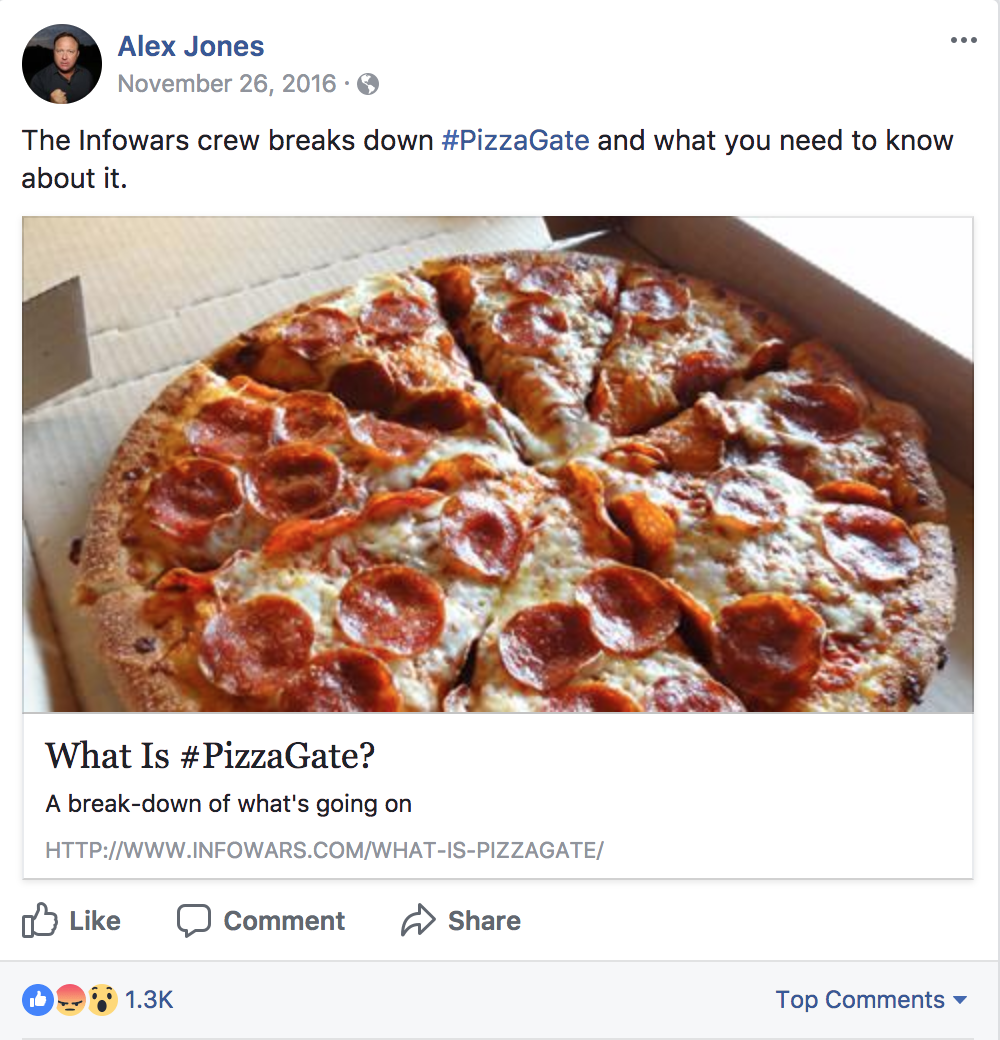
\includegraphics[scale=.3]{pizzagate_alex_jones_fb}
	\end{minipage}
	\begin{minipage}{0.48\textwidth}
		\centering
		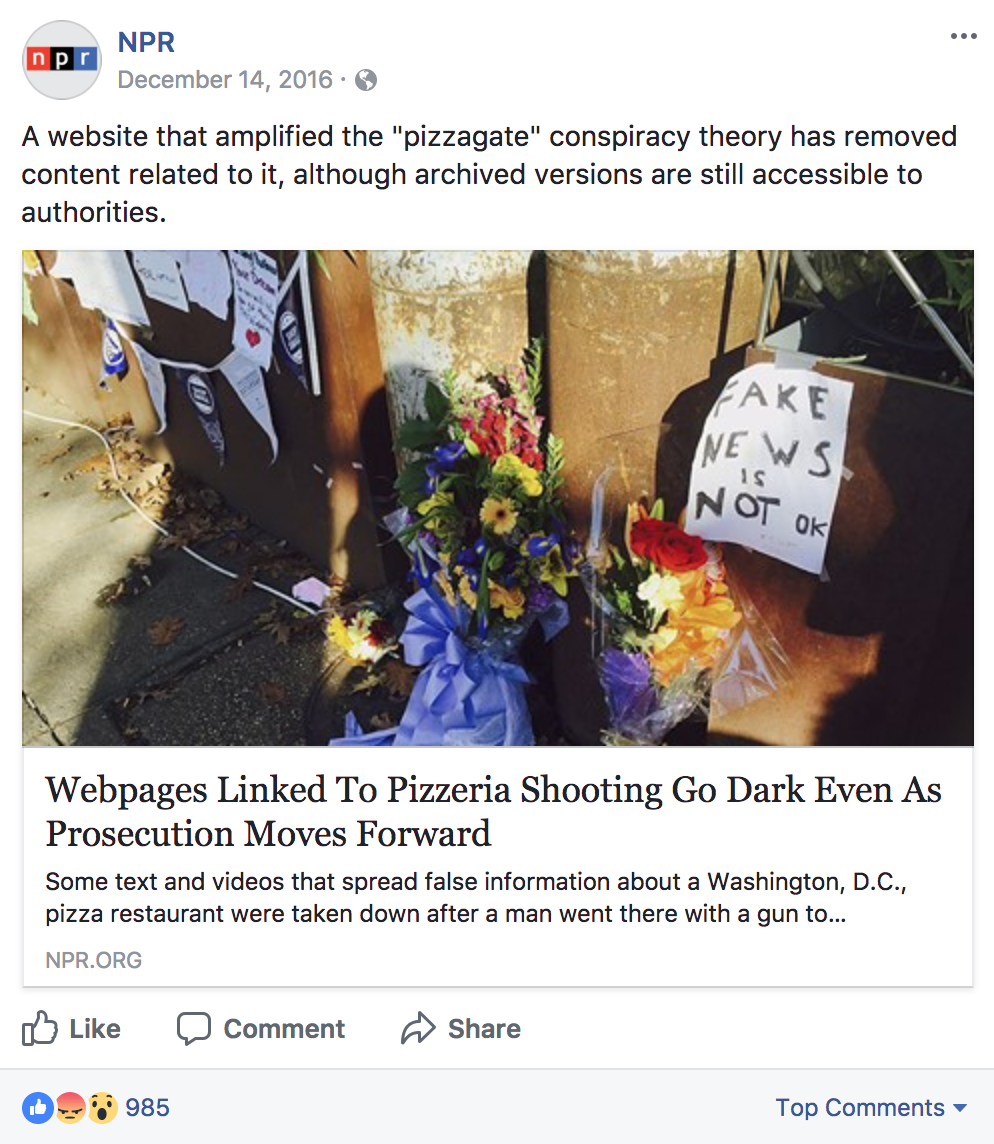
\includegraphics[scale=.3]{pizzagate_npr_fb}
	\end{minipage}
	\caption{A comparison of posts by Alex Jones, creator of {\it Infowars}, \citep{alex_jones_pizzagate_post} and {\it NPR} \citep{npr_pizzagate_post} about Pizzagate.}
\end{figure}

This uniform formatting treats {\it NPR} and {\it Infowars} or any other site that uses the \texttt{meta} elements according to Facebook's specifications as equals. It places less emphasis on the source of the article than on the headline and picture. The examples above are posted from official accounts, allowing users to easily see where the article comes from. However, the same articles posted by friends or unofficial pages make the source more difficult to determine. In addition, 50\% of shared links generate less than 1\% of clicks on social media \citep{clicks_vs_shares}, meaning most shares happen without the user clicking the link and reading the article. Therefore what a user sees on Facebook's preview is most likely all that user sees and is entirely determined by the web developer, with the possibility that the headline, picture, and description are totally unrelated to the actual content of the article, factually incorrect, or telling an attention-grabbing but incomplete story.

If Facebook were to put more focus on the content of the article rather than the title, this would reduce the negative utility generated by misleading or inaccurate articles being shared based on preview content that is entirely separate from what is inside the link itself. Automatic summarization is a potential solution, where an automatically generated summary is added to the preview, possibly in place of the description section created by the author. This forces the text shown in the preview to be more representative of the actual content the user would read if they were to click on the article. An alternative would be to take the contents of the article itself and place a truncated version into the preview content on a user's feed. This would be easily understood by users with a short explanation, and potentially aid in users understanding the contents of the article before they share, minimizing the impact and negative utility generated by misleading headlines.

Facebook could resolve this by implementing an automatic summarization of the contents of the page, however summarizing text has many technical hurdles. Automated summarization of text is an active area of research in natural language processing and even evaluating the quality of summaries in relation to longer pieces of text is often unclear. Summarizing often requires context for concepts, objects, or people mentioned and a system summarizing based off only the text presented to it can write summaries as misleading as what would have been in it's place without the automatic system. The truncated text could be subject to loopholes when gathering the text and potentially rife with abuse. Web developers could easily put misleading descriptions in text that is invisible on the page or only load text content from a server rather than being embedded in the page for Facebook's web crawler.

\section{Age of the Article: Hannah}

Considering the age of the article is an important aspect of identifying fake news. Both very recent articles and older articles can be subject to scrutiny. Older articles can be brought back lacking any date other than the age of the post using Facebook's link previewing feature or quoted by newer articles out of context with no means of cross referencing, manipulating a potential reader into thinking an article is relevant to a current situation in addition to whether they are factually accurate. Likewise, news articles that rapidly accumulate reactions, shares, and likes can appear on an unmoderated trending topics list, regardless of the content of the article. On October 1, 2017, a man opened fire on a crowd attending a concert in Las Vegas, killing 59 people and injuring over 500. Almost instantly, fake news began to spread about the topic, reaching the top of trending pages across the internet, including Facebook. The articles and posts varied in topics, ranging from flooding social media with posts falsely searching for missing relatives, calling the shooter an Islamic convert and the shooting an act of Islamic terror, or saying the shooter was involved with Antifa and had attended anti-Trump rallies \citep{buzzfeed_vegas_conspiracies}. All of these false statements were posted and promoted in a way that was meant to disrupt the flow of accurate information or make those seeking help less able to find it. Actions perpetrated by 4chan and other internet message boards were actively malicious, with no intentions other than to sow chaos and spread often bigoted lies about victims and the perpetrator alike. Actively impeding those who sought to help in Las Vegas, those searching for missing friends and family, and anyone looking for information about the tragedy creates an enormous amount of negative utility for every user who is not actively participating in the misinformation campaign by being less likely to find the resources they were looking for.

Situations like the Las Vegas shooting pose a difficult challenge for Facebook. In chaotic situations, important information can be gained from an individual's posts online, particularly before traditional media arrives. However it is not clear until much later what posts are real and which are outright lies. In the instances where fake posts searching for family were posted by personal accounts, included pictures were often of lesser known or regionally unknown celebrities, such as foreign soccer players. Fake posts of this type will increase negative utility for people trying to help locate missing people, however limiting or preventing posts of this type might create more negative utility from angry and concerned friends and family of those near the incident. However, limiting blog posts and unverified news sources from reaching the trending topics list until a certain time after the event might be a way to minimize negative utility for other users who would be looking for information on the incident but not otherwise looking to attack.

Facebook has recently implemented the ability for users to ``check in" safe after a variety of events from around the world in an attempt to stem the flood of fake posts searching for friends and family without impeding anyone from actually making the posts, however the effectiveness of this system is not known. Anyone who does not hear from someone they care about may still post in search of that person, leaving the door still open for fake posts to flood a user's feed. Limiting content on the trending topics list immediately surrounding to verified accounts is very feasible for Facebook, however making a verified account more difficult to get would be necessary or a different verification process for news stories or media companies would need to be developed. One potential would be to only allow trending topics from news sources with a high percentage of their content being previously verified. This could allow networks with a history of good behavior to get their stories to be seen without any interaction with developing stories themselves.

While an enormous amount of negative utility is generated on Facebook every time an incident like the Las Vegas shooting happens, determining what is real and what is fake is not clear, even to potential human curators, let alone algorithmic curators. The negative utility earned from implementing a bad classifier for filtering personal user's posts could easily generate far more negative utility than was initially created by the fake posts themselves. Fake or unverified news stories reaching trending lists might be easier to control with less potential negative utility generated from mistakes as long as Facebook develops a method of curation that filters out unverifiable sources, such as message forums and blog posts. 

\section{Article Genre: Hannah}

the onion, dedicated satire site, https://www.theonion.com/no-way-to-prevent-this-says-only-nation-where-this-r-1819580358

new yorker, sometime satire, 

"just a joke" defense for harassment, 



\section{Interpretation Bias: Hannah}
Facebook recently came under fire for their manual curation of trending news topics when former Facebook employees were interviewed by Gizmodo about the trending news section. One curator said ``There was no real standard for measuring what qualified as news and what didn't" and that they regularly avoided right wing sites such as \textit{Breitbart} and \textit{The Blaze}. When pressed for a comment, Facebook responded by claiming they ``take allegations of bias very seriously" \citep{gizmodo_fb_news_curation}. By framing bias as a negative, Facebook implies that they view themselves as a neutral entity and that they believe it is possible for the website and trending topics to be free of bias.


trending topic staff fired, https://www.theguardian.com/technology/2016/aug/29/facebook-fires-trending-topics-team-algorithm



\section{Cross reference with fact-checking sites: Zane}
The next method for assisting in classifying fake news on Facebook is to implement fact checking for an article. This involves using a web crawler to go around and potentially fact check that sites. More precisely, in an ideal scenario, when a user posts a link on Facebook, the page linked to should have been indexed, and there should be a metric associated with the page that conveys the trustworthiness of the content presented. If the score falls below a particular threshold, Facebook may deprioritize the link.  

From a utilitarian perspective, we feel that on the surface, this method seems like it has the potential to greatly hinder the spread of fake news. If the content on a page is primary false, then deprioritizing it hinders it getting around the web. The major downside we see is that often, the articles linked to on Facebook are not formally written scholarly articles, but rather more casual ones. In these types of articles, opinions are presented as facts, and vice-versa. This creates an ambiguity in how we define a fact. We feel that in this case, even if there existed an NLP oracle that could perfectly distinguish fact from opinion, the majority of articles would be flagged as false negative simply because of people's writing style. Overall, what little positive utility that this brings would be quickly overshadowed by negative utility.

In terms of the technical feasibility, the same argument can be made here. From an NLP perspective, it would be challenging enough to even write a method that could parse the text and pull out statements, let alone distinguish fact from opinion. Additionally, the context of the statement would need to go through sentiment analysis to determine the authors intentions for even writing the comment in the first place. For this reason, we feel that Facebook attempting to distinguish fact from opinion is technically infeasible, and because of this, would result in in an increase in the negative utility.

\section{Supporting sources: Zane}
The final method for identifying fake news is to check supporting sources (if any) and make sure they abide by the same rules. In other words, this method attacks the problem with a recursive approach. When a user wants to share an article on the site, the fake news classification algorithm could take a depth first approach at calculating a trustworthiness metric. This can be done by first calculating the trustworthiest of the sources linked to in the article, and then using this metric in the overall trustworthiness calculation for the main article.

From a utilitarian perspective, where our main goal is to minimize the amount of negative utility brought about by fake articles, we feel that implementing this method has a few angles to look at the problem from. The core idea of this method is to first apply the other methods that we feel are appropriate. We next take a depth first approach, using these metrics to generate a metric for the primary article. We feel that for the most part, this would be an extra step in minimizing the spread of fake news. One point to keep in mind however is that by taking a recursive approach, we may be rating the credibility of one page based on the credibility of a page with multiple degrees of separation that have virtually nothing to do with each other. Also, as mentioned in \textit{Credible sites and Sources}, there doesn't exist a reliable algorithm to to flag a link with the context that it's being cited in. For example, if an author is citing a fake news article with the intention of pointing out the fake news, sentiment analysis would need to be implemented so that the trustworthiness metric would somehow understand this context, and not use this against the articles score.

In terms of the technical feasibility of the implementation, there are a few issues that would make this point difficult to implement. The first hurdle is that there would have to be some kind of standardization to the method that sites use to track citations and references. Most sites that people read have a nonstandard citations section at the bottom of the page that consists of random bits of metadata and URLs. Although this conveys the required information to the \textit{reader}, it fails to be parsable by a web crawler. Additionally, this depth first approach to calculating source credibility would involve storing a large amount of metadata.

\section{Conclusion}

With the increasing veracity of fake news across all of social media, particularly Facebook, and the consequences of letting misinformation spread rapidly and unchallenged, Facebook has an ethical responsibility to come up with an effective and equitable strategy to combat its spread. Additionally, a Pew Research Center survey found 68\% of Facebook users get news from Facebook, but only 33\% of Facebook users get news from local TV or dedicated news sites and apps \citep{pew_news}. Facebook earns more than twice the engagement in news than any single non-social media platform but Facebook does not hold itself to any standard for the integrity of their sources unlike most traditional formats. Because of its large impact on users, Facebook has an ethical obliation to attempt to stop the spreading of fake news among its users. 

As we've seen in our analysis of the methods of inhibiting fake news, there are many challenges involved in implementing these tactics. Not only are some of these methods technically infeasible, but implementing them in algorithm form may open up the doors to more negative utility than it actually stops. Additionally, with the volume of posts shared, it is not possible Facebook to tackle these problems manually with human intervention. Algorithmic intervention seems to be the most practical solution if human moderation and automatic moderation were equally accurate, however there are just as many different struggles for developing an algorithmic fake news detection system. The primary issues that we see arising come down to privacy concerns, interpreting an author's motivations, and automatic fact checking.

If Facebook were to decide to invest in an automated system for detecting fake news, they will need to be transparent at every step of the process. In order to begin designing such a system, Facebook needs to determine what they value in a news source and be willing to stand by those beliefs in the face of adversity or openly change them in response to criticism. Their negative response towards ``allegations of bias" in response to not allowing a site that frequently promotes white nationalism, fake news, and harassment campaigns, \textit{Brietbart}, onto the trending topics list, they are themselves making a political statement in tacit support of the platform's message by treating its inadvertent suppression as a something to be corrected, which conflicts with previous statements against hate speech and harassment. Neutrality is not apolitical. \textbf{more stuff}

\newpage
%\bibliographystyle{apalike}
%\bibliography{proposal_bibliography.bib}
\printbibliography

\end{document}
